\documentclass{article}

\usepackage[margin=1in]{geometry}
\usepackage{listings}
\usepackage{color}
\usepackage{graphicx}
\usepackage{float}

\definecolor{dkgreen}{rgb}{0,0.6,0}
\definecolor{gray}{rgb}{0.5,0.5,0.5}
\definecolor{mauve}{rgb}{0.58,0,0.82}

\lstset{frame=tb,
	language=C,
	aboveskip=3mm,
	belowskip=3mm,
	showstringspaces=false,
	columns=flexible,
	basicstyle={\small\ttfamily},
	numbers=left,
	numberstyle=\color{gray},
	keywordstyle=\color{blue},
	commentstyle=\color{dkgreen},
	stringstyle=\color{mauve},
	breaklines=true,
	breakatwhitespace=true,
	tabsize=4
}

\title{Lab 7: Serial Communication(SPI and I2C)}
\date{November 06, 2017}
\author{Matthew Friedman 861151348\\Souradeep Bhattacharya 861105938\\EE128 Section: 021}
\begin{document}
	\maketitle
	\section*{Abstract}
	The objective of this lab was to get familiar with SPI and I2C programming. Both of these techniques allow us to add additional functionality to our microcontroller.
	\section*{Experimental System Specification}
	\subsection*{Part 1: SPI based I/O Extender MCP23S08}
	In this lab experiment, we will obtain 3-bit information from a switch and display this info by using the lower 3 LEDs. Then we will change the order in which the LEDs light up relative to the switch. Then finally we will switch the location of the switch and LEDs on the I/O expander.
	\subsection*{Part 2: I2C-based EEPROM Interfacing and Programming}
	In this lab experiment we will write a two 8 byte pages to the EEPROM and then read them back to make sure it was written correctly.
	\section*{Block Diagram}
	\subsection*{Part 1: SPI based I/O Extender MCP23S08}
	\begin{figure}[H]
		\centering
		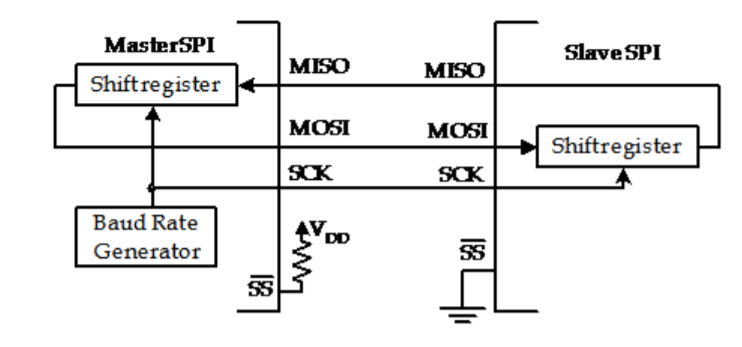
\includegraphics[scale=0.75]{SPI_BD_1}
		\caption{SPI Shift Register Diagram}
	\end{figure}
	\begin{figure}[H]
		\centering
		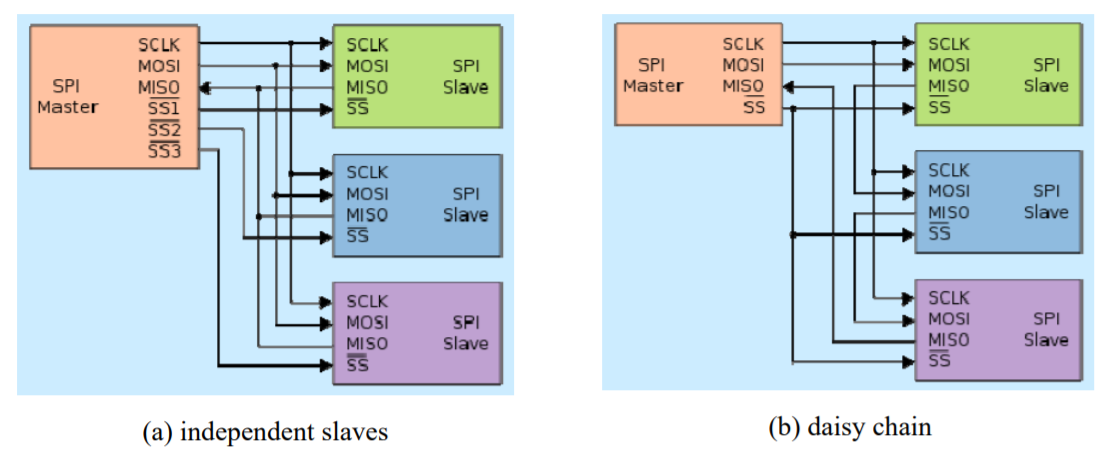
\includegraphics[scale=0.75]{SPI_BD_2}
		\caption{SPI Block Diagram}
	\end{figure}
	\subsection*{Part 2: I2C-based EEPROM Interfacing and Programming}
	\begin{figure}[H]
		\centering
		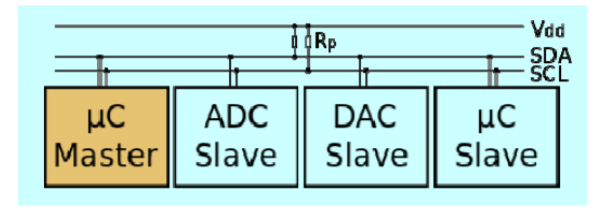
\includegraphics[scale=0.75]{I2C_BD}
		\caption{SPI Block Diagram}
	\end{figure}

	\section*{Detailed Schematic}
	\subsection*{Part 1: SPI based I/O Extender MCP23S08}
	\begin{figure}[H]
		\centering
		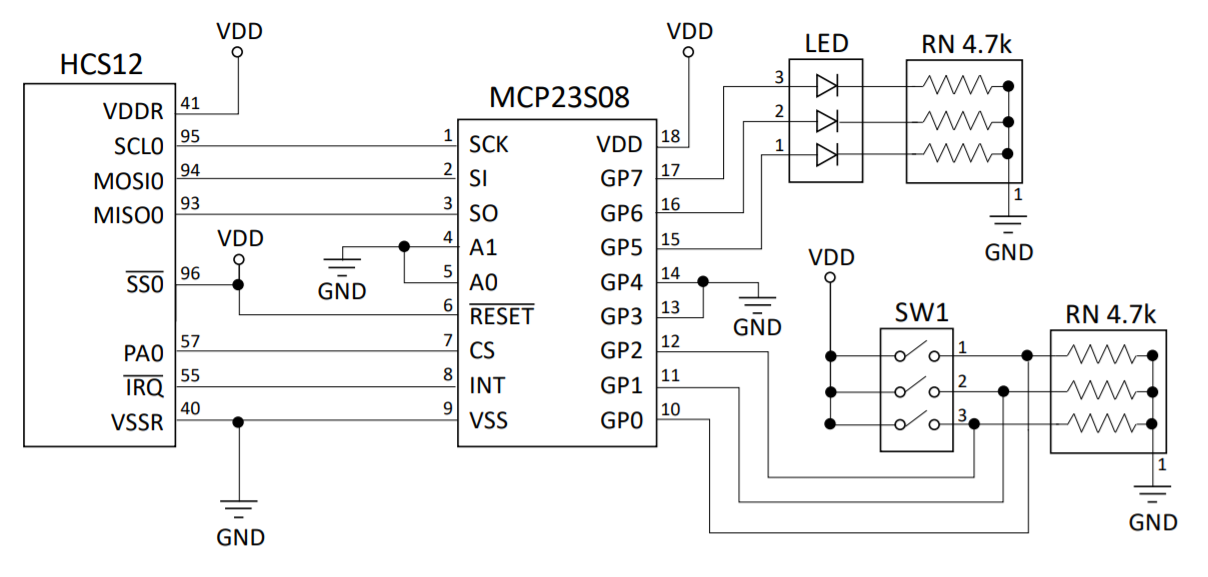
\includegraphics[scale=0.75]{SPI_SCH}
		\caption{SPI Detailed Diagram}
	\end{figure}
	\subsection*{Part 2: I2C-based EEPROM Interfacing and Programming}
	\begin{figure}[H]
		\centering
		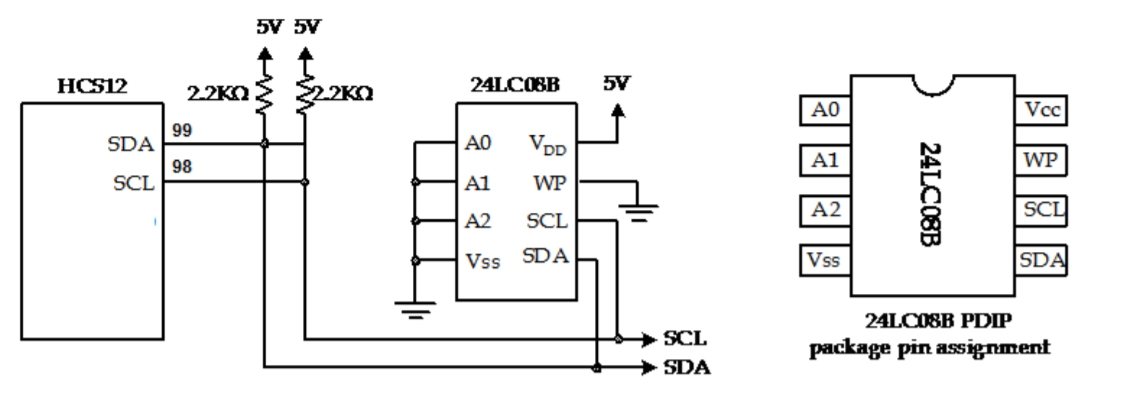
\includegraphics[scale=0.75]{I2C_SCH}
		\caption{I2C Detailed Diagram}
	\end{figure}
	\section*{High Level Description of Software}
	\subsection*{Part 1: SPI based I/O Extender MCP23S08}
	This device first had to be configured before it could be used properly. We modified the template give to us to enabled it to to what we wanted it to.
	\subsection*{Part 2: I2C-based EEPROM Interfacing and Programming}
	This particular EEPROM had a default page size of 8-bytes and supported page-writing. The command was exactly the same as the normal write command except you do not send the stop condition until after 8 pages had been written. It would handle the auto incrementing of the addresses. We simply did this twice to write the two pages. 
	\section*{Program Listing}
	\subsection*{Part 1: SPI based I/O Extender MCP23S08}
	\begin{lstlisting}
	/* ********************************************************************** *
	*  Project:     SPI_IO_Expander                                          *
	*  Purpose:     EE128 Lab 7, SPI and I2C Communication                   *
	*                                                                        *
	*  Notes:       1. See Lab 7 manual for a detailed testbench schematic   *
	*               2. Switches are supposed to be initially ALL OFF         *
	* ********************************************************************** */
	
	#include <hidef.h>         /* common defines and macros */
	#include <mc9s12dg256.h>   /* derivative information */
	#include "spi.h"           /* MC9S12 SPI Library */
	#include "mcp23s08.h"      /* I/O Expander Registers and Bits */
	
	#define  INPORT      0x00     /* INPUT  Port */
	#define  OUTPORT     0xFF     /* OUTPUT Port */
	
	char temp = 0x00;
	
	extern void putcspi0(char);
	extern void putsspi0(char*);
	extern char getcspi0(void);
	extern void getsspi0(char*, char);
	
	void          SPI_SetIOXregister(unsigned char,unsigned char);
	unsigned char SPI_GetIOXregister(unsigned char); 
	
	__interrupt void IRQISR(void);
	
	static unsigned char regByte; /* temporal variable for register data */
	
	#define  IOX_WR_OP  0x40   /* R/W bit = 0, address is always hardware 00 (grounded) */
	#define  IOX_RD_OP  0x41   /* R/W bit = 1, address is always hardware 00 (grounded) */
	
	/* ****************************************************************** *
	*                                                                    *
	*                                 MAIN                               *
	*                                                                    *
	* ****************************************************************** */
	
	void main(void) {
	
	/* ****************************************************************** *
	*                                                                    *
	*                            SETUP                                   *
	*                                                                    *
	* ****************************************************************** */
	
		DDRA = OUTPORT;  /* control \CS pin of IOX chip */
		PORTA = 0x01;    /* initially deselect IOX chip */
	
	/*** Setup MC9S12 Interrupt Service ***/
	
		PORTE = 0x02;    /* IRQ PIN PE1 PULL HIGH */
		INTCR = 0xC0;    /* enable IRQ interrupt on falling edge */
		asm("cli");      /* enable interrupt globally */
	
	/*** Setup MC9S12 SPI Module ***/
	
		SPI0BR  = 0x77;  /* set baudrate to the minimum possible 11.719 kHz*/
		SPI0CR1 = 0x50;  /* enable SPI, master mode, disable interrupt, SCK idle low,
	data shift on SCK's rising edge, CPHA=0 */
		SPI0CR2 = 0x02;  /* disable bidirectional mode, SPI stops in wait mode */
		WOMS    = 0;     /* enable Port S pull-up; otherwise use external resistors for pull-up */
	
	/*** Setup MCP23S08 I/O Expander Registers ***/
	
		regByte = 0x78;  /* GP7..GP5 - output (LED's); GP2..GP0 - 	input (switches) */
		SPI_SetIOXregister(IOX_IODIR,regByte);
	
		regByte = 0xF0;  /* enable interrupt-on-change for GP2..GP0 */
		SPI_SetIOXregister(IOX_GPINTEN,regByte);
	
	/*** Setup Initial Output in I/O output pins ***/
	
		regByte = 0x00;  /* set zero initial output values */
		SPI_SetIOXregister(IOX_GPIO,regByte);
	
	/* ****************************************************************** *
	*                                                                    *
	*                             LOOP                                   *
	*                                                                    *
	* ****************************************************************** */
	
		for(;;){} // wait for interrupts caused by switch changes
	
	}   /* main */
	
	/* ****************************************************************** *
	*                                                                    *
	*                       INTERRUPT ROUTINES                           *
	*                                                                    *
	* ****************************************************************** */
	
	__interrupt void IRQISR(void)
	/* interrupt routine to set new LED/Oscilloscope outputs */
	{
		regByte = SPI_GetIOXregister(IOX_GPIO);
		regByte >>= 4;
		temp = regByte;
		//regByte = ((temp & 0x80) >> 7) | ((temp & 0x40) >> 5) | ((temp & 0x20) >> 3);  
		SPI_SetIOXregister(IOX_GPIO,regByte);
	}
	
	/* ****************************************************************** *
	*                                                                    *
	*                    AUXILIARY SPI ROUTINES                          *
	*                                                                    *
	* ****************************************************************** */
	
	void SPI_SetIOXregister(unsigned char ioxAddress,
	unsigned char regValue   ) {
		/* Write-Op to set registers,
	and using PTA0 pin of PORTA to control CS pin of IOX */
	
		PORTA = 0x00;          /* chip select, using PORTA */
		putcspi0(IOX_WR_OP);   /* schedule a writing op to a register */
		putcspi0(ioxAddress);  /* write to the address of IODIR register */
		putcspi0(regValue);    /* write to IODIR register */  
		PORTA = 0x01;          /* chip diselect */
	
	}
	
	unsigned char SPI_GetIOXregister(unsigned char ioxAddress) {
		/* Read-Op to read registers,
	and using PTA0 pin of PORTA to control CS pin of IOX */
	
		unsigned char regValue;
	
		PORTA = 0x00;          /* chip select using PORTA */
		putcspi0(IOX_RD_OP);   /* schedule a writing op to a register */
		putcspi0(ioxAddress);  /* write to the address of IODIR 	register */
		regValue = getcspi0(); /* write to IODIR register */  
		PORTA = 0x01;          /* chip diselect */
	
		return regValue;
	}
	\end{lstlisting}
	\subsection*{Part 2: I2C-based EEPROM Interfacing and Programming}
	\subsubsection*{I2C Header}
	\begin{lstlisting}
	/* ************************************************* *
	*         I2C Library for EEPROM 24LC01B            *
	* ************************************************* */
	
	#include <hidef.h>
	#include <stdio.h>
	#include <mc9s12dg256.h>
	#include "i2c.h"
	
	//#define DBG_ON 
	
	/* OpenI2C */
	void Init_I2C (char ibc, char I2C_ID)
	{
	#ifdef DBG_ON
		printf("9S12: Configure I2C\r\n");
	#endif
		IBCR |= IBEN;          /* enable I2C module */
		IBFD = ibc;            /* set up I2C baud rate */
		IBAD = I2C_ID;         /* set up I2C slave address */
		IBCR &= ~IBIE;         /* disable I2C interrupt */
		IBCR |= IBSWAI;        /* disable i2C in wait mode */
	}
	
	/* SendSlaveID */
	void SendSlaveID(char cx)
	{
	
	#ifdef DBG_ON
		printf("I2C: 9S12 Send Slave ID\r\n");
	#endif
		while(IBSR & IBB);     /* wait until I2C bus is idle */
	
	#ifdef DBG_ON
		printf("I2C:     Bus is Idle\r\n");
	#endif
	
	#ifdef DBG_ON
		printf("I2C: 9S12 Generate Start condition\r\n");
	#endif
	
		IBCR |= TXRX + MSSL;   /* generate a start condition */
		IBDR = cx;             /* send out slace ID with R/W set to 0 */
		while(!(IBSR & IBIF)); /* wait for completion of transmission */
	
	#ifdef DBG_ON
		printf("I2C: 9S12 Start condition ... OK\r\n");
	#endif
	
		IBSR = IBIF;           /* clear IBIF flag */
	
	#ifdef DBG_ON
		printf("I2C: 9S12 Send Slave ID ... done\r\n");
	#endif
	}
	
	//#define DBG_ON_R
	
	/* EERandomRead */
	char EErandomRead(char ID, char addr)
	{
		char dummy;
	
	#ifdef DBG_ON_R
		printf("I2C: 9S12 Read a byte from EEPROM\r\n");
	#endif
	
		SendSlaveID(ID);
	
	#ifdef DBG_ON_R
		printf("I2C:9S12 Wait for Transmission Acknowledgment\r\n");
	#endif
		if (IBSR & RXAK)       /* wait for transmission ackn	nowledgment */
			return -1;
	#ifdef DBG_ON_R
		printf("I2C:EEPROM ... Ack\r\n");
	#endif
	
	#ifdef DBG_ON_R
		printf("I2C: 9S12 Send Address\r\n");
	#endif
		IBDR = addr;           /* send out EEPROM address */
	
		while(!(IBSR & IBIF)); /* wait util the address is sent out */
	
		IBSR = IBIF;           /* clear IBIF flag */
	
		if (IBSR & RXAK)
			return -1;
	
	#ifdef DBG_ON_R
		printf("I2C: EEPROM ... Ack\r\n");
	#endif
	
	#ifdef DBG_ON_R
		printf("I2C: 9S12 Generate Restart condition and prepare to read\r\n");
	#endif
		IBCR |= RSTA;          /* generate restart condition */
		IBDR = ID | 0x01;      /* prepare to read */
	
		while (!(IBSR & IBIF));
	
		IBSR = IBIF;
		if (IBSR & RXAK)
		return -1;
	#ifdef DBG_ON_R
		printf("I2C: EEPROM ... Ack\r\n");
	#endif
	
		IBCR |= TXAK;  /* prepare to send NACK */
		IBCR &= ~TXRX; /* perform reception */
	#ifdef DBG_ON_R
		printf("I2C:9S12 Trigger 9 clock pulses to read\r\n");
	#endif
		dummy = IBDR;  /* dummy read to trigger 9 clock pulses */
		while(!(IBSR & IBIF)); /* wait for data to shift in */
	#ifdef DBG_ON_R
		printf("I2C: EEPROM Send Byte... OK\r\n");
	#endif
		IBSR = IBIF;
		IBCR &= ~MSSL; /* generate a stop condition */
	#ifdef DBG_ON_R
		printf("I2C: 9S12 Generate Stop condition and finish reading a byte\r\n");
	#endif
		return IBDR;
	}
	
	/* EEbyteWrite */
	char EEbyteWrite(char ID, char addr, char data)
	{
	
	#ifdef DBG_ON
		printf("I2C: 9S12 Write a byte to EEPROM\r\n");
	#endif
	
	#ifdef DBG_ON
		printf("I2C: 9S12 Wait for Acknowledgment\r\n");
	#endif
		SendSlaveID(ID);
	
		if (IBSR & RXAK) /* error if EEPROM does not acknowledge */
			return -1;
	#ifdef DBG_ON
		printf("I2C: EEPROM ... Ack\r\n");
	#endif
	
	#ifdef DBG_ON
		printf("I2C: 9S12 Send Address\r\n");
	#endif
		IBDR = addr;     /* send out address of the location to be written */
		while(!(IBSR & IBIF));
		IBSR = IBIF;     /* clear the IBIF flag */
		if (IBSR & RXAK) /* error if EEPROM does not acknowledge */
			return -1;
	#ifdef DBG_ON
		printf("I2C: EEPROM ... Ack\r\n");
	#endif
	
	#ifdef DBG_ON
		printf("I2C: 9S12 Send Data\r\n");
	#endif
		IBDR = data;     /* send out the data byte */
		while(!(IBSR&IBIF));
		IBSR = IBIF;     /* clear the IBIF flag */
		if (IBSR & RXAK) /* error if EEPROM does not respond */
			return -1;
	#ifdef DBG_ON
		printf("I2C: EEPROM ... Ack\r\n");
	#endif     
	
		IBCR &= ~MSSL;   /* generate a stop condition */
	#ifdef DBG_ON
		printf("I2C: 9S12 Generate Stop condition and finish reading a byte\r\n");
	#endif
		return 0;        /* normal write code */
	}
	
	/* eeAckPoll */
	void eeAckPoll(char ID)
	{
		SendSlaveID(ID);
		while(IBSR & RXAK){
		IBCR |= RSTA;   /* generate a restart condition */
		IBDR = ID;      /* send out EEPROM ID */
		while(!(IBSR & IBIF));
			IBSR = IBIF;    /* clear the IBIF flag */
		} ; /* continue if EEPROM did not acknowledge */
		IBCR &= ~MSSL;     /* generate a stop condition */
	}
	
	/* EEbyteWrite */
	char EEPageWrite(char ID, char addr, char * data)
	{
		char i;
	#ifdef DBG_ON
		printf("I2C: 9S12 Write a byte to EEPROM\r\n");
	#endif
	
	#ifdef DBG_ON
		printf("I2C: 9S12 Wait for Acknowledgment\r\n");
	#endif
		SendSlaveID(ID);
	
		if (IBSR & RXAK) /* error if EEPROM does not acknowledge */
			return -1;
	#ifdef DBG_ON
		printf("I2C: EEPROM ... Ack\r\n");
	#endif
	
	#ifdef DBG_ON
		printf("I2C: 9S12 Send Address\r\n");
	#endif
		IBDR = addr;     /* send out address of the location to be written */
		while(!(IBSR & IBIF));
		IBSR = IBIF;     /* clear the IBIF flag */
		if (IBSR & RXAK) /* error if EEPROM does not acknowledge */
			return -1;
	#ifdef DBG_ON
		printf("I2C: EEPROM ... Ack\r\n");
	#endif
	
	//#ifdef DBG_ON
		printf("I2C: 9S12 Send Data\r\n");
	//#endif
		for(i = 0; i < 8; i++) {
	
		IBDR = data[i];     /* send out the data byte */
		while(!(IBSR&IBIF));
		IBSR = IBIF;     /* clear the IBIF flag */
		if (IBSR & RXAK) /* error if EEPROM does not respond */
	return -1;
	
	//#ifdef DBG_ON
			printf("I2C: EEPROM ... Ack\r\n");
	//#endif     
		}
		IBCR &= ~MSSL;   /* generate a stop condition */
	#ifdef DBG_ON
		printf("I2C: 9S12 Generate Stop condition and finish reading a byte\r\n");
	#endif
		return 0;        /* normal write code */
	}
	\end{lstlisting}
	\subsubsection*{Main}
	\begin{lstlisting}
	/* ********************************************************************** *
	*  Project:     I2C_EEPROM                                               *
	*  Purpose:     EE128 Lab 7, SPI and I2C Communication                   *
	*                                                                        *
	*  Notes:       See Lab 7 manual for a detailed testbench schematic      *
	* ********************************************************************** */
	
	#include <hidef.h>
	#include <stdio.h>
	#include <mc9s12dg256.h>
	#include "i2c.h"
	
	
	#define DBG_ON                /* print out debugging information if enabled */
	
	
	void clearscreen(void)
	{
		putchar(0x0C);
	}
	
	void main(void) {
	
		const char *msgMemo = "I2C based EEPROM Reading and Writing";
		char rd;
		char memchar = 0x00;
		
		char eeprom_address = 0x0A;  /* address in EEPROM to write a byte to */
		char eeprom_data    = 0x05;  /* data byte to be written to EEPROM */
		
		char data1[8] = {0x01,0x02,0x04,0x08,0x01,0x02,0x04,0x08};
		char data2[8] = {0x0a,0x0b,0x0c,0x0d,0x0d,0x0c,0x0b,0x0a};
		
		char i;
		
		clearscreen();
		printf("EE128 LAB 7\r\n");
		printf("I2C based EEPROM Reading and Writing\r\n");
		
		printf("**************************************\r\n");
		printf("   9S12 will write a byte to EEPROM\r\n   ");
		printf("**************************************\r\n");
		printf("EEPROM address: 0x%x\r\n", eeprom_address); 
		printf("EEPROM data:    0x%x\r\n", eeprom_data);
	
	#ifdef DBG_ON
		printf("- running in DEBUG mode -\r\n");
	#endif
	
		Init_I2C(0x1F,0xFE);         /* configure I2C module */
		
		rd = EEbyteWrite(0xA0,eeprom_address,eeprom_data);
		eeAckPoll(0xA0);            /* make sure internal write operation is complete */
		
		printf("\r\n");    
		printf("***************************************\r\n");
		printf("   9S12 will read a byte from EEPROM\r\n");
		printf("***************************************\r\n");
		
		memchar = EErandomRead(0xA0,eeprom_address);
		
		printf("EEPROM @ 0x%x = 0x%x\r\n", eeprom_address, memchar);
		
		eeprom_address = 16; 
		
		printf("\r\n");    
		printf("***************************************\r\n");
		printf("   9S12 will write pages to EEPROM\r\n");
		printf("***************************************\r\n");
		
		EEPageWrite(0xA0, eeprom_address, data1);
		eeAckPoll(0xA0);
		EEPageWrite(0xA0, eeprom_address + 8, data2);
		eeAckPoll(0xA0);
		
		printf("\r\n");    
		printf("***************************************\r\n");
		printf("   9S12 will read pages back EEPROM\r\n");
		printf("***************************************\r\n");
	
		for(i = 0; i < 16; i++) {
	
		printf("Reading Data %d ", i);
			memchar = EErandomRead(0xA0,eeprom_address+i);
	
			printf("EEPROM @ 0x%x = 0x%x\r\n", eeprom_address+i, 	memchar);
		}
	
	
		for(;;) {} /* wait forever */
	}
	
	\end{lstlisting}
	
	\section*{Technical Problems}
	There were no major technical problems encountered.
	\section*{Conclusion}
	In this lab we successfully used two very common serial communication protocols. They showed us how we can extend our I/O and how we can store data in non volatile memory.
\end{document}